% ****** Start of file apssamp.tex ******
%
%   This file is part of the APS files in the REVTeX 4.2 distribution.
%   Version 4.2a of REVTeX, December 2014
%
%   Copyright (c) 2014 The American Physical Society.
%
%   See the REVTeX 4 README file for restrictions and more information.
%
% TeX'ing this file requires that you have AMS-LaTeX 2.0 installed
% as well as the rest of the prerequisites for REVTeX 4.2
%
% See the REVTeX 4 README file
% It also requires running BibTeX. The commands are as follows:
%
%  1)  latex apssamp.tex
%  2)  bibtex apssamp
%  3)  latex apssamp.tex
%  4)  latex apssamp.tex
%
\documentclass[%
 reprint,
%superscriptaddress,
%groupedaddress,
%unsortedaddress,
%runinaddress,
%frontmatterverbose, 
%preprint,
%preprintnumbers,
%nofootinbib,
%nobibnotes,
%bibnotes,
 amsmath,amssymb,
 aps,
%pra,
prb,
%rmp,
%prstab,
%prstper,
%floatfix,
]{revtex4-2}

\usepackage{graphicx}% Include figure files
\usepackage{dcolumn}% Align table columns on decimal point
\usepackage{bm}% bold math
\usepackage{hyperref}% add hypertext capabilities
\usepackage{verbatim}
\usepackage[capitalise]{cleveref}
\usepackage[skins,theorems]{tcolorbox}
\tcbset{highlight math style={enhanced,colframe=red,colback=white,arc=0pt,boxrule=1pt}}
%\usepackage[mathlines]{lineno}% Enable numbering of text and display math
%\linenumbers\relax % Commence numbering lines

%\usepackage[showframe,%Uncomment any one of the following lines to test 
%%scale=0.7, marginratio={1:1, 2:3}, ignoreall,% default settings
%%text={7in,10in},centering,
%%margin=1.5in,
%%total={6.5in,8.75in}, top=1.2in, left=0.9in, includefoot,
%%height=10in,a5paper,hmargin={3cm,0.8in},
%]{geometry}

\begin{document}

\preprint{APS/123-QED}

\title{Notes on ionic water}% Force line breaks with \\
%\thanks{A footnote to the article title}%


\newcommand{\ai}{\textit{ab initio} }

%\author{Stefano Baroni}
% \altaffiliation[Also at ]{Physics %Department, XYZ University.}%Lines %break automatically or can be forced %with \\
\author{Davide Tisi}%
 \email{dtisi@sissa.it}
\affiliation{%
 SISSA\\
 This line break forced with \textbackslash\textbackslash
}%

%\collaboration{MUSO Collaboration}%\noaffiliation

%\author{Charlie Author}
%\homepage{http://www.Second.institution.edu/~Charlie.Author}
%\affiliation{
% Second institution and/or address\\
% This line break forced% with \\
%}%
%\affiliation{
% Third institution, the second for Charlie Author
%}%
%\author{Delta Author}
%\affiliation{%
% Authors' institution and/or address\\
% This line break forced with \textbackslash\textbackslash
%}%

%\collaboration{CLEO Collaboration}%\noaffiliation
\newcommand{\FS}{F^{\star}}

\date{\today}% It is always \today, today,
             %  but any date may be explicitly specified

\begin{abstract}
The following are some notes on the results of ionic water with NN
\end{abstract}

%\keywords{Suggested keywords}%Use showkeys class option if keyword
                              %display desired
\maketitle

%\tableofcontents
\section{Introduction}
We used some data of partial dissociated water (PDL) to fit a NN potential with DeepMD code \cite{Linfeng2018,Wang2017}. Before to analyse the statical, dynamical and conduction properties we show  in \cref{table:thermo} the thermodynamic conditions of the two simulations.

\begin{table}[h]
\begin{tabular}{ c c c c }
\hline
  &$\rho$ & T & P  \\
 &g/cm$^3$ &K &GPa  \\
\hline
 \ai &2.04&$1970 \pm 60$ & $33 \pm 1$ \\
 DeepMD &2.03& $2013 \pm 60$ & $30.0 \pm 1.3 $ \\
 \hline 
\end{tabular}
\caption{Summary of the thermodynamical conditions of the two simulations \ai and with NN potential  }
\label{table:thermo}
\end{table}

The NN simulation has a average temperature a bit higher but the pressure is slightly lower (\textbf{not compatible}).
In the following sections we can compare the different staticala and dynamical properties: the radial distribution function (gofr), the vibrational density of state (VDOS), the electrical and thermal conductivity.
\section{GOFR}
The first and easiest property to check is the radial distribution function, both \ai and NN results are obtained from a $100~$ps trajectory. The static properties are very well reproduced, in fact \cref{fig:GOFR} shows the gofr computed from the \ai and NN trajectory, the results are in good agreement and are compatible for any $r$.

\begin{figure}[tbh]
    \centering
    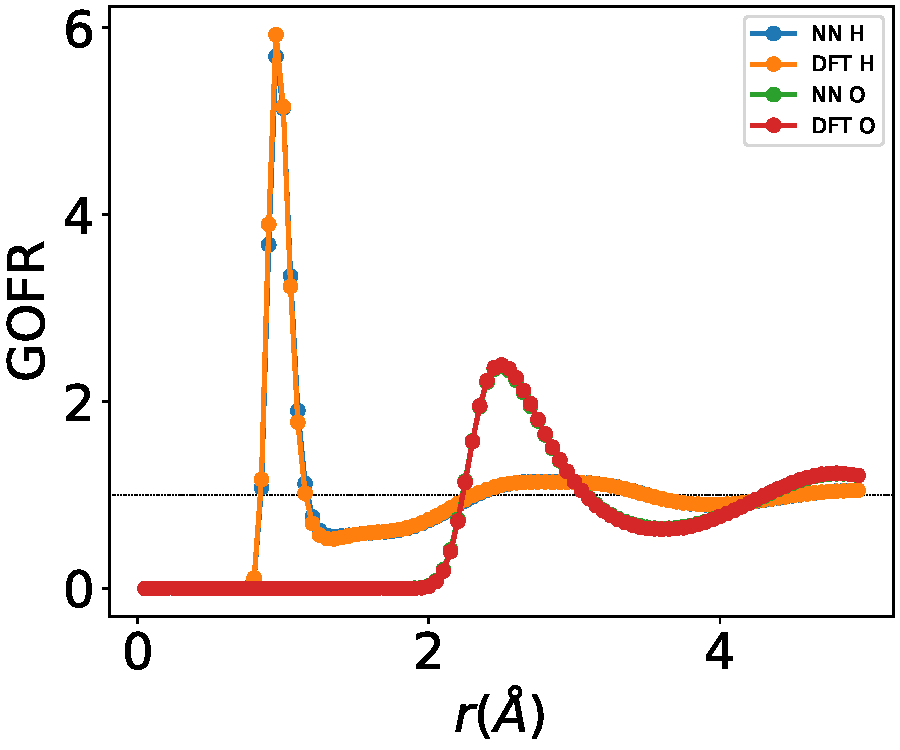
\includegraphics[width=\linewidth]{figs/GOFR.pdf}
    \caption{Comparison between gofr computed from the \ai (blue lines) and DeepMD (red lines) trajectories, both $100~$ps long. The results are compatible for all the distances.} 
    \label{fig:GOFR}
\end{figure}

\section{VDOS}
The second properties we can analyse is the vibrational density of states (VDOS), a dynamical properties which gives us the self-diffusion coefficient, or diffusivity, for $\omega=0$:
\begin{align}
\text{VDOS}_{\alpha}(\omega) =& \frac{1}{3N_{\alpha}}\sum_{i=0}^{N_{\alpha}}\int_{-\infty}^{\infty} \langle \mathbf{v}_i(0)\mathbf{v}_i(t) \rangle_{\text{eq}}~ e^{i \omega t} dt \\
D_{\alpha} = & \frac{1}{2}\text{VDOS}_{\alpha}(\omega = 0),
\end{align}
where $N_{\alpha}$ is the total number of atoms of the species $\alpha$. 

\begin{figure}[tbh]
    \centering
    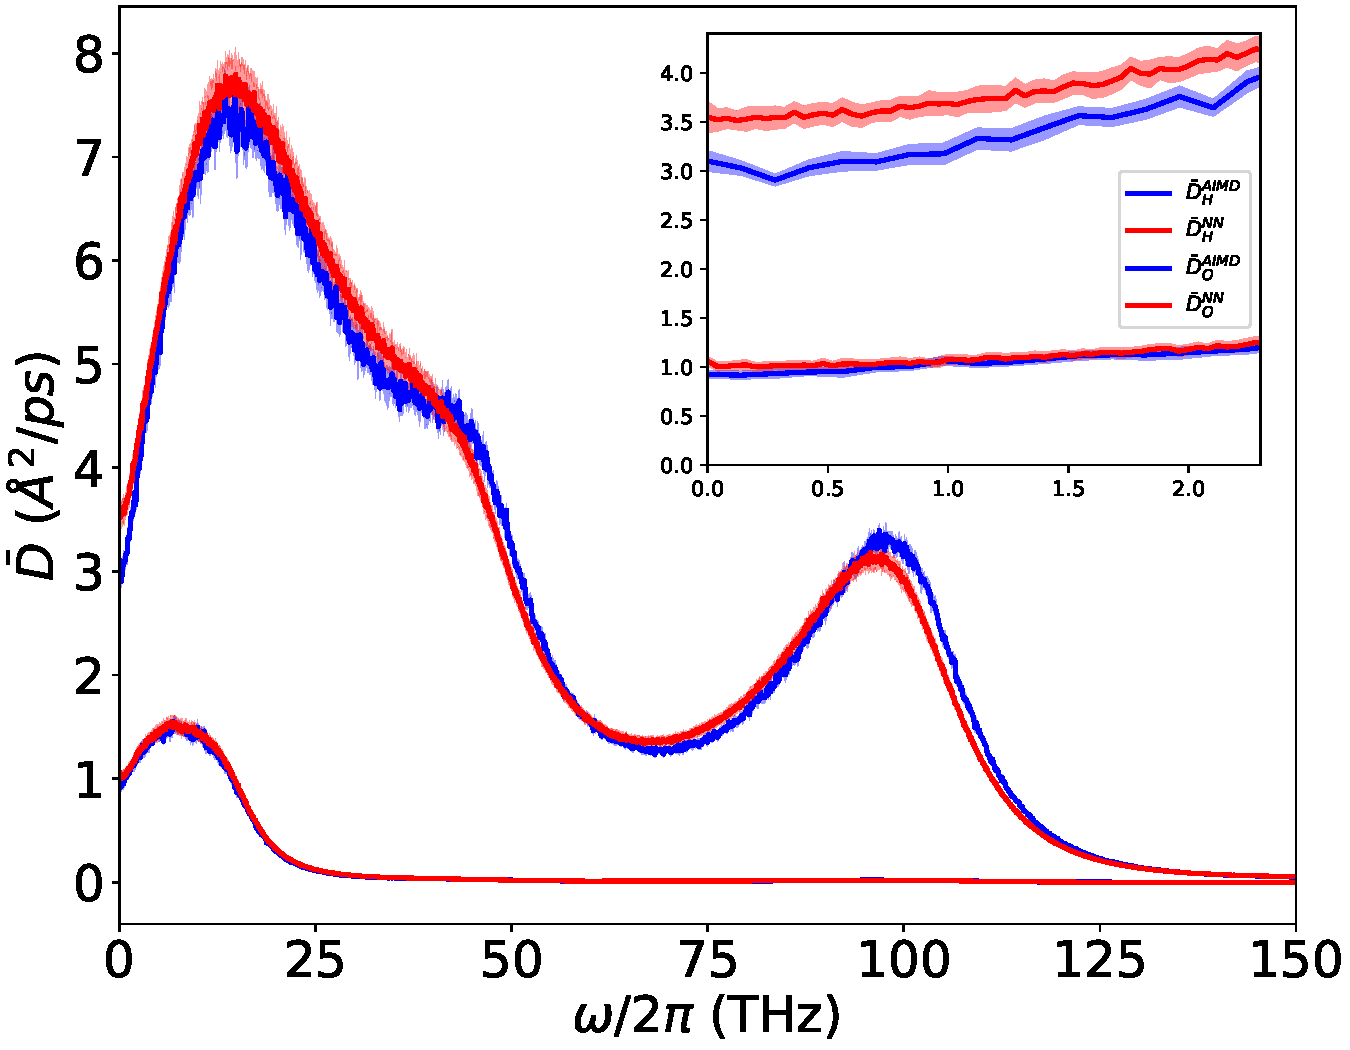
\includegraphics[width=\linewidth]{figs/VDOS.pdf}
    \caption{$\bar{D}(\omega) = \frac{1}{2}\text{VDOS}(\omega)$ for both \ai (blue lines) and DeepMD (red lines) trajectories, respectively $100~$ps and $900~$ps long. The self-diffusivity, $\bar{D}_{\alpha}(\omega=0)$ are not consistent and the NN gives always an higher diffusivity.}
    \label{fig:VDOS}
\end{figure}

\cref{fig:VDOS} shows  $\bar{D}(\omega)=\frac{1}{2}\text{VDOS}(\omega)$ computed with the \ai and DeepMD trajectory, while for oxygens the results are quite compatible, for hydrogens the two spectra have slightly different features, in particular at zero the spectra are not consistent, leading to different values of self-diffusivity: $\bar{D}_{H}^{\text{AIMD}}=3.10 \pm 0.10$,  $\bar{D}_{H}^{\text{NN}}=3.55 \pm 0.15$, $\bar{D}_{O}^{\text{AIMD}}=0.92 \pm 0.04$ and $\bar{D}_{O}^{\text{NN}}=1.06  \pm 0.05$.

\section{Electrical conductivity }\label{sec:El_cond}
The electrical conductivity $\sigma$ is computed as the zero-frequency value of the power spectrum of the following charge flux:
\begin{equation}
\mathbf{J}_Z = q_H \sum_{i \in H}\mathbf{v_i} + q_O \sum_{i \in O}\mathbf{v_i},
\end{equation}
where $\mathbf{v}_i$ is the atomic velocity of $i$-th atom, while the atomic charges are equal to the integer oxidation numbers $q_H = +1$ and $q_O = -2$.


\begin{figure}[tbh]
    \centering
    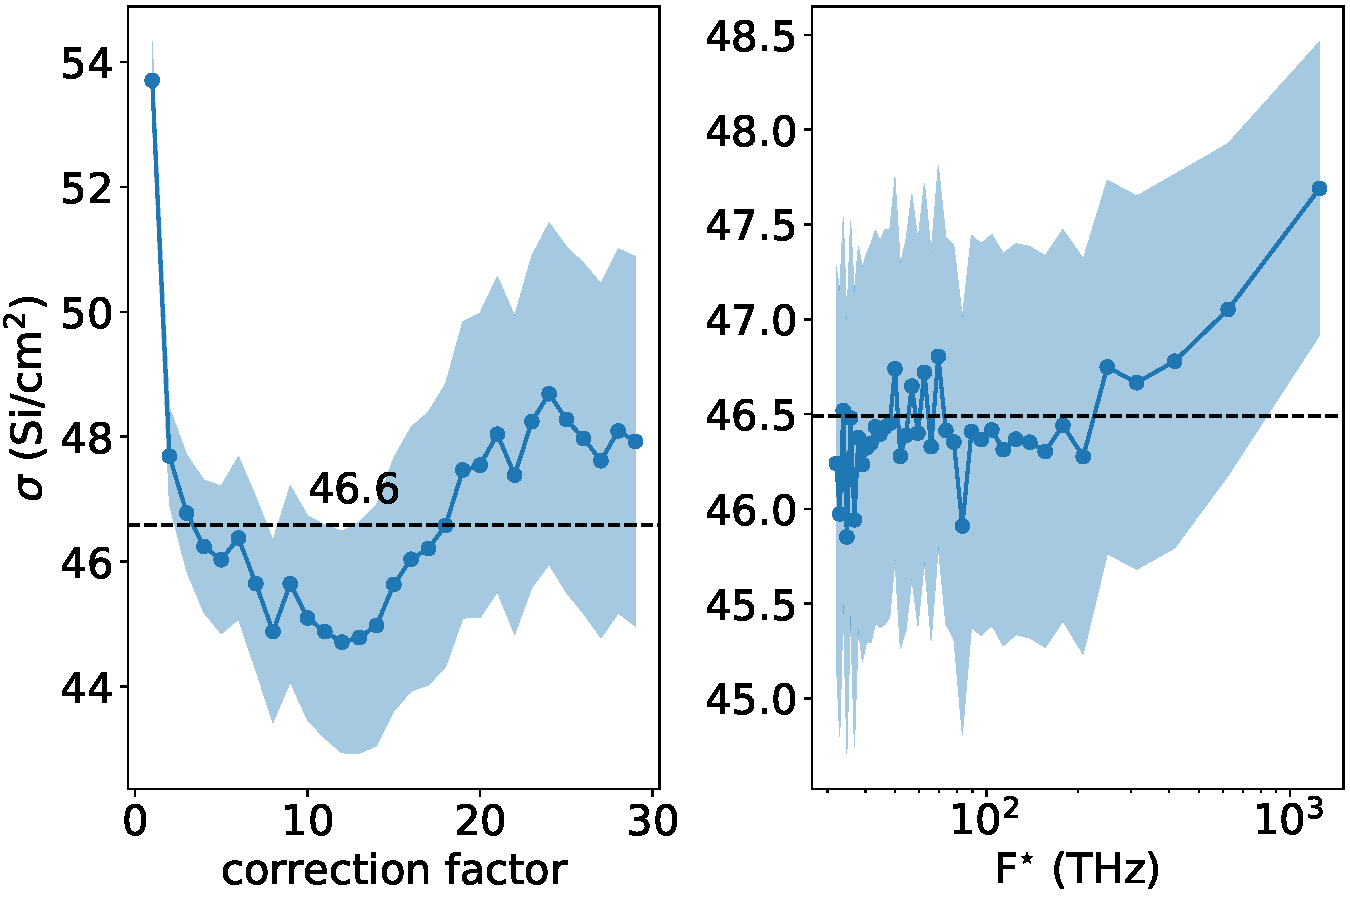
\includegraphics[width=\linewidth]{figs/sigma.pdf}
    \caption{Dependence of $\sigma$ from the corrector factor, $c$, to the AIC criterion (left panel) and from $F^{\star}$ (right panel). The black dotted lines are the mean values. All the results of the right panel are obtained with  $c=2$, which is the one that, in the right panel, has the smallest number of $P^{\star}$ between those which give $\sigma$ consistent with the average. }
    \label{fig:sigma}
\end{figure}

The estimates and uncertainties of $\sigma$ are obtained via cepstral analysis. \cref{fig:sigma} shows the dependence of $\sigma$ from the corrector factor, $c$, (left panel) and $F^{\star}$ (right panel). For $c > 1$ all the values of $\sigma$ are consistent with each other, so for the $F^{\star}$ analysis we employed $c=2$, which gives us the smallest number of $P^{\star}$ .
From the right panel of \cref{fig:sigma} we can see that $\sigma$ do not depend on $F^{\star}$ and so we can decide an "optimal" value of $F^{\star}$: $\sigma^{NN}(F^{\star}=50)=46.7 \pm  1.0 ~$S/cm consistent with the \ai value $\sigma^{AIMD}=45 \pm  5 ~$S/cm

\section{Thermal conductivity}
The thermal conductivity is computed as the zero-frequency value of the heat flux:
\begin{equation}
\mathbf{J} = \frac{1}{\Omega}\left[\sum_i \varepsilon_i \mathbf{v}_i + \sum_{i,j} (r_i-r_j) \frac{\partial u_i}{\partial r_j}v_j \right]
\end{equation}
where $\varepsilon_i$ are the atomic contribution to the total energies $\sum_i \varepsilon_i =E=K+U$ and $\sum_i u_i =U$. \cref{fig:kappa} shows the behaviour of $\kappa$ as function of $\FS$ for many values of $c$, for $c>1$ all the results are consistent with each other so, in order to minimize the error we can chose $c=2$ and then  $\FS=57$, that leads us to:
$\kappa^{NN} = 4.09 \pm 0.09~$W/(mK) consistent with the \ai value $\kappa^{AIMD} = 4.2 \pm 0.3~$W/(mK) 

\begin{figure}[tbh]
    \centering
    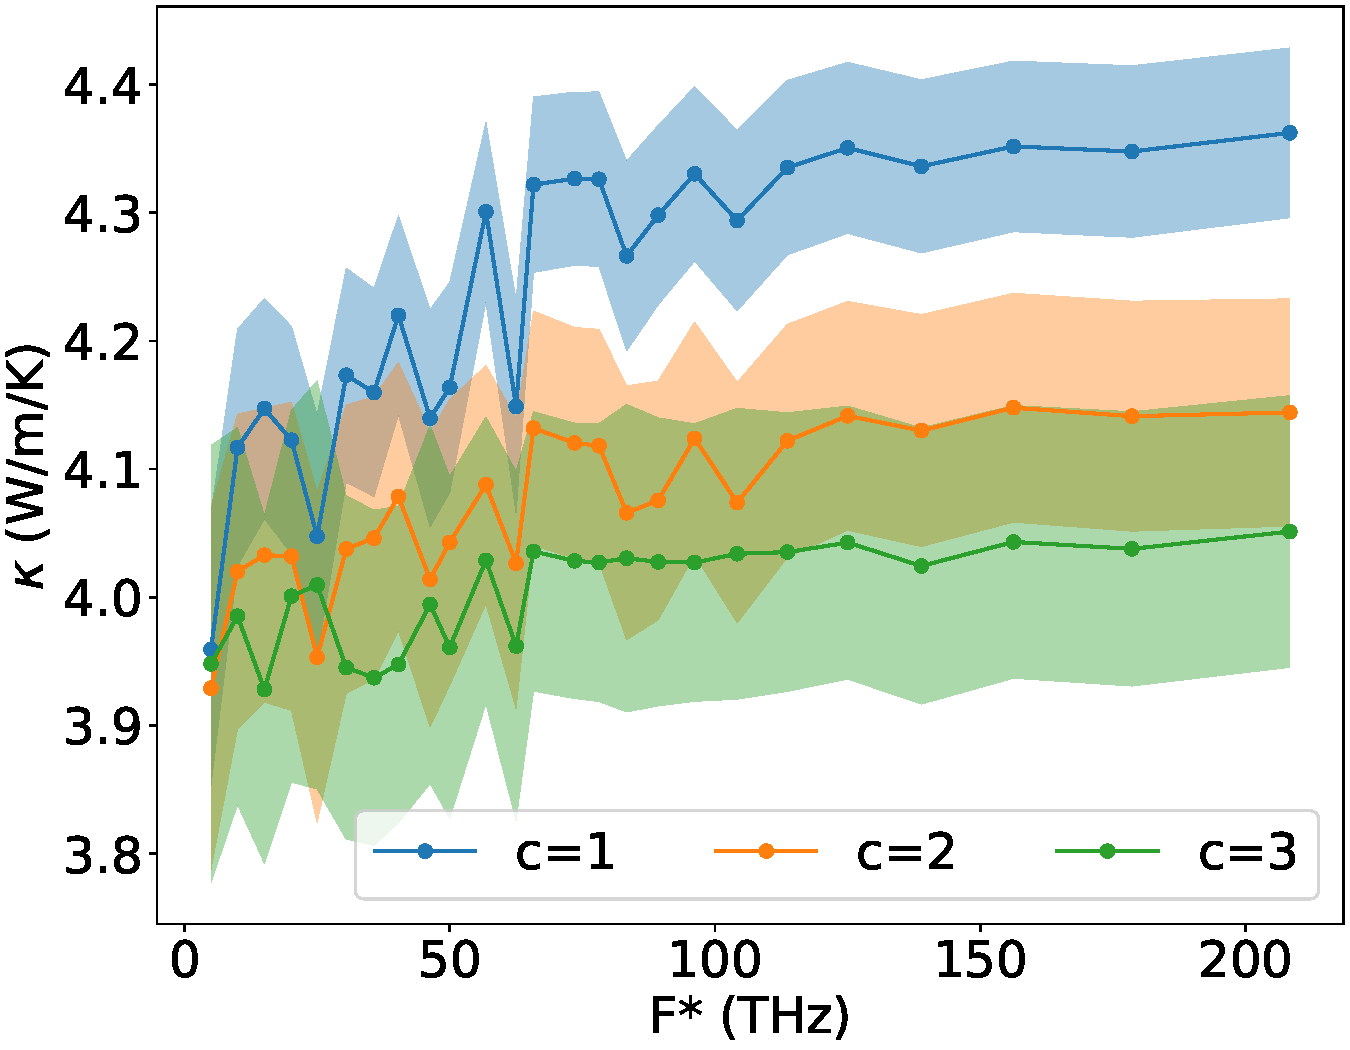
\includegraphics[width=\linewidth]{figs/kappa_corr_Fstar.pdf}
    \caption{Value of $\kappa$ as function  of $\FS$ for different values of $c$. }
    \label{fig:kappa}
\end{figure}


%\appendix
\section{Conclusion}

\cref{table:results} summarizes and compares the results for the \ai and DeepMD simulation.

\begin{table}[h]
\begin{tabular}{ c  c  c  c  c  c  c  }
\hline
  &$\kappa$ &  $\sigma$ &$D_{H(O)}$ &$\rho$ & T & P  \\
 &W/(mK)&S/cm &\AA$^2$ / ps & g/cm$^3$ &K &GPa  \\
\hline
 \ai & $4.2\pm 0.3$ & $45 \pm 5$ &$3.10\pm 0.10$& 2.04&$1970 \pm 60$ & $33 \pm 1$ \\
      &    &   & $0.92 \pm 0.04$  &  &  &  \\
 DeepMD & $4.09 +\- 0.09 $ & $46.7 \pm 1.0$ &$3.55\pm 0.15$ &2.03& $2013 \pm 60$ & $30.0 \pm 1.3 $ \\
       &    &   & $1.06 \pm 0.05$  &  &  &  \\
 \hline 
\end{tabular}
\caption{Summary of the results of the two simulations \ai and with NN potential  }
\label{table:results}
\end{table}


\section{Second simulation}
We trained a new model with a different number of parameters, a fitting network with 4 layers with 300, 250, 200, 100 neurons respectively. After performing a simulation with the new potential we can compare the three results:
from AIMD, from the first NN (which will be labeled NN$_0$) and from the second NN (which will be labeled NN$_1$).
In the beginning we can compare again the thermodynamic conditions:

\begin{table}[h]
\begin{tabular}{ c c c c }
\hline
  &$\rho$ & T & P  \\
 &g/cm$^3$ &K &GPa  \\
\hline
 \ai &2.04&$1970 \pm 60$ & $33 \pm 1$ \\
 $NN_0$ &2.03& $2013 \pm 60$ & $30.0 \pm 1.3 $ \\
 $NN_1$ &2.03& $1967 +/- 58$ & $22.8 +/- 1.3 $ \\
 \hline 
\end{tabular}
\caption{Summary of the thermodynamical conditions of the three simulations: \ai , with NN$_0$ and with NN$_1$ potential. }
\label{table:thermo_1}
\end{table}

Again all the thermodynamic parameters are compatible except the pression that is quite low.
\cref{fig:GOFR1,fig:VDOS1} show the result for the gofr and the VDOS, respectively. The latter is similar in all the cases but at zero they gives a different value of the diffusivity, in particular for NN$_1$ (black line): $\bar{D}_{H}^{\text{NN}_1}=3.36 \pm 0.18 $ and $\bar{D}_{O}^{\text{NN}_1}=0.97 \pm 0.04$.
\begin{figure}[tbh]
    \centering
    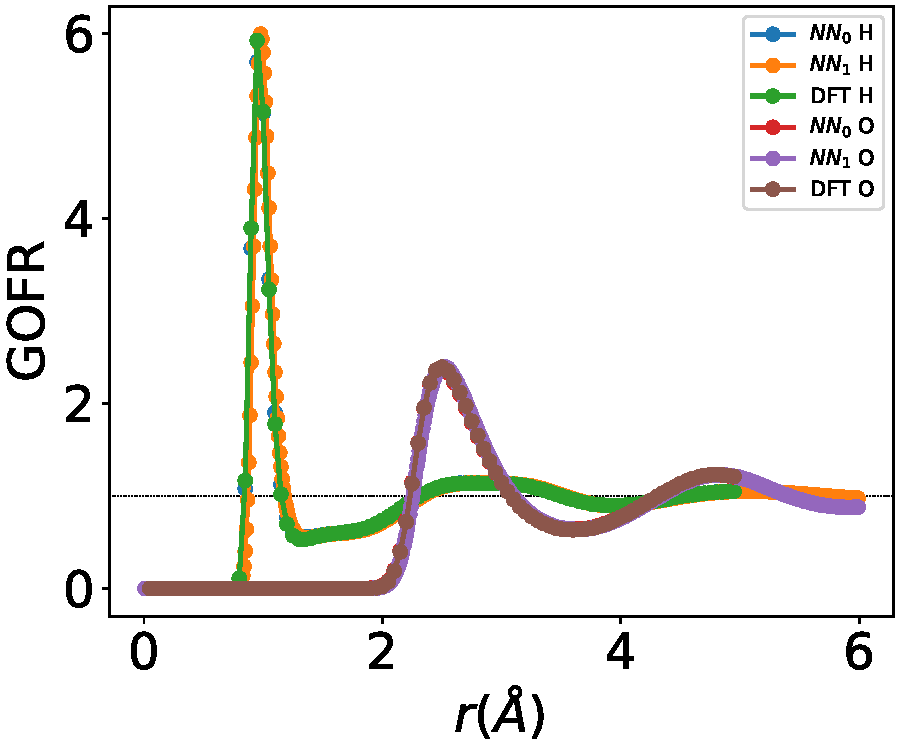
\includegraphics[width=\linewidth]{figs/GOFR_all.pdf}
    \caption{Comparison between gofr computed from the \ai (blue lines), NN$_0$ (red lines), NN$_1$ (black line) trajectories, both $100~$ps long. The results are compatible for all the distances.} 
    \label{fig:GOFR1}
\end{figure}

\begin{figure}[bt]
    \centering
    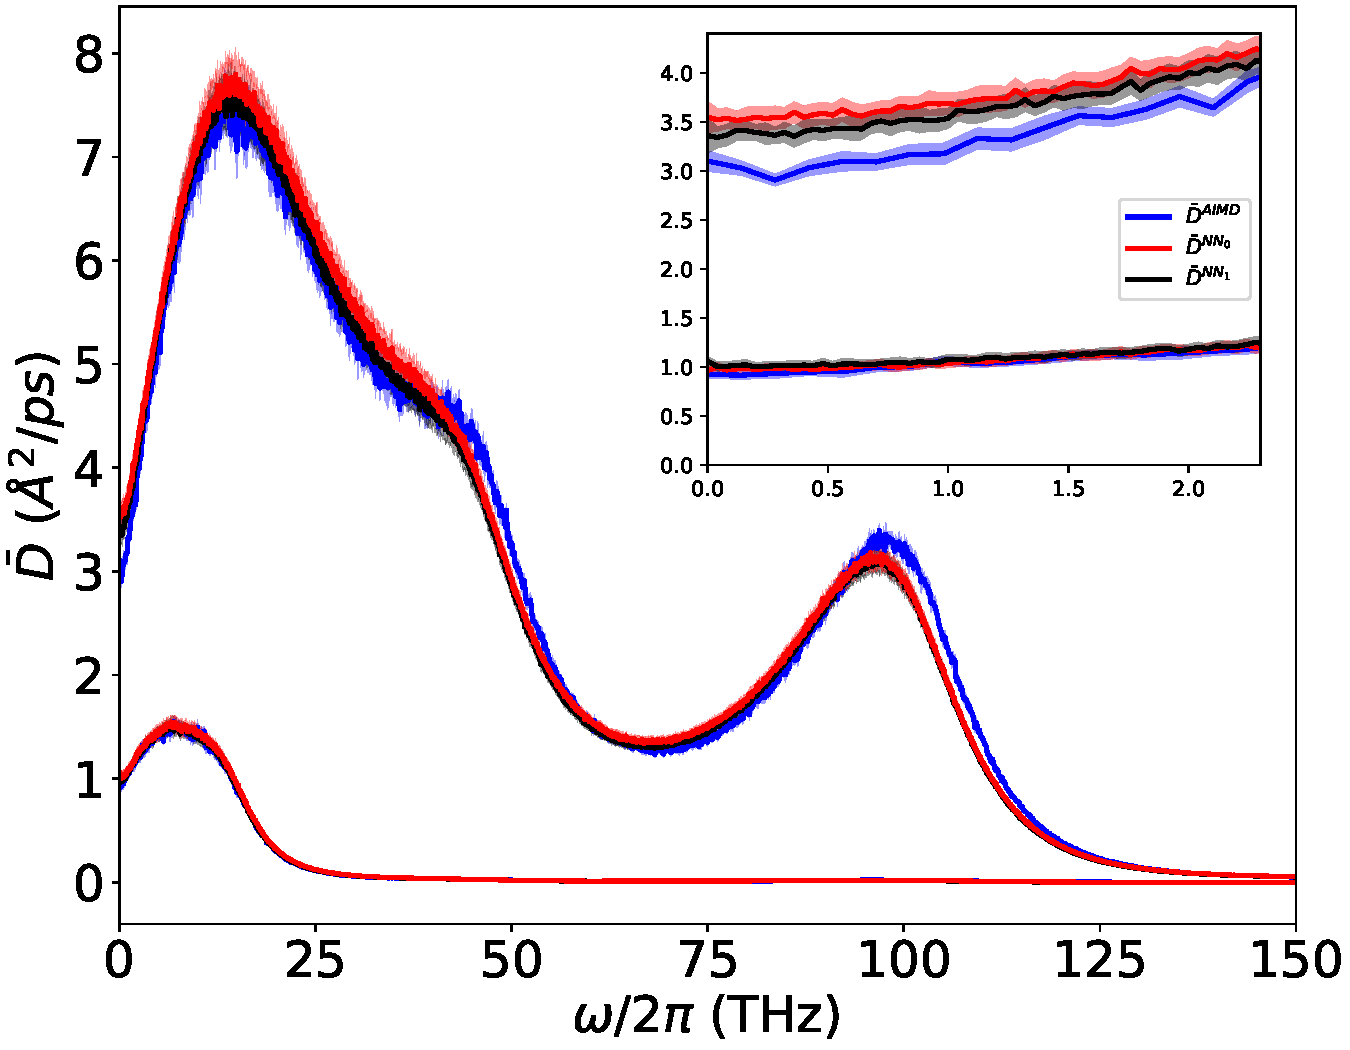
\includegraphics[width=\linewidth]{figs/VDOS_all.pdf}
    \caption{$\bar{D}(\omega) = \frac{1}{2}\text{VDOS}(\omega)$ for \ai (blue lines), NN$_0$ (red lines), NN$_1$ (black lines) trajectories, respectively $100~$ps, $900~$ps and $900~$ps long. The self-diffusivity, $\bar{D}_{\alpha}(\omega=0)$ are not consistent and the NN gives always an higher diffusivity.} 
    \label{fig:VDOS1}
\end{figure}

The analysis of the charge properties are the same of section \cref{sec:El_cond}, so we will report only the result in the final table. Now we pass to the thermal transport properties, again we analyse $\kappa$ as function of $c$ and $\FS$ (\cref{fig:kappa1}). We choose $c=2$ and $\FS=55$, thus $\kappa^{\text{NN}_1}=3.35 \pm 0.09$, not consistent with the value obtained from both\ai and NN$_0$. \cref{fig:spettri} shows the power spectrum for simulation NN$_0$ (orange) and NN$_1$, we can see that event for window-filtered spectra (shadow regions) NN$_0$ is higher than NN$_1$.

\begin{figure}[tbh]
    \centering
    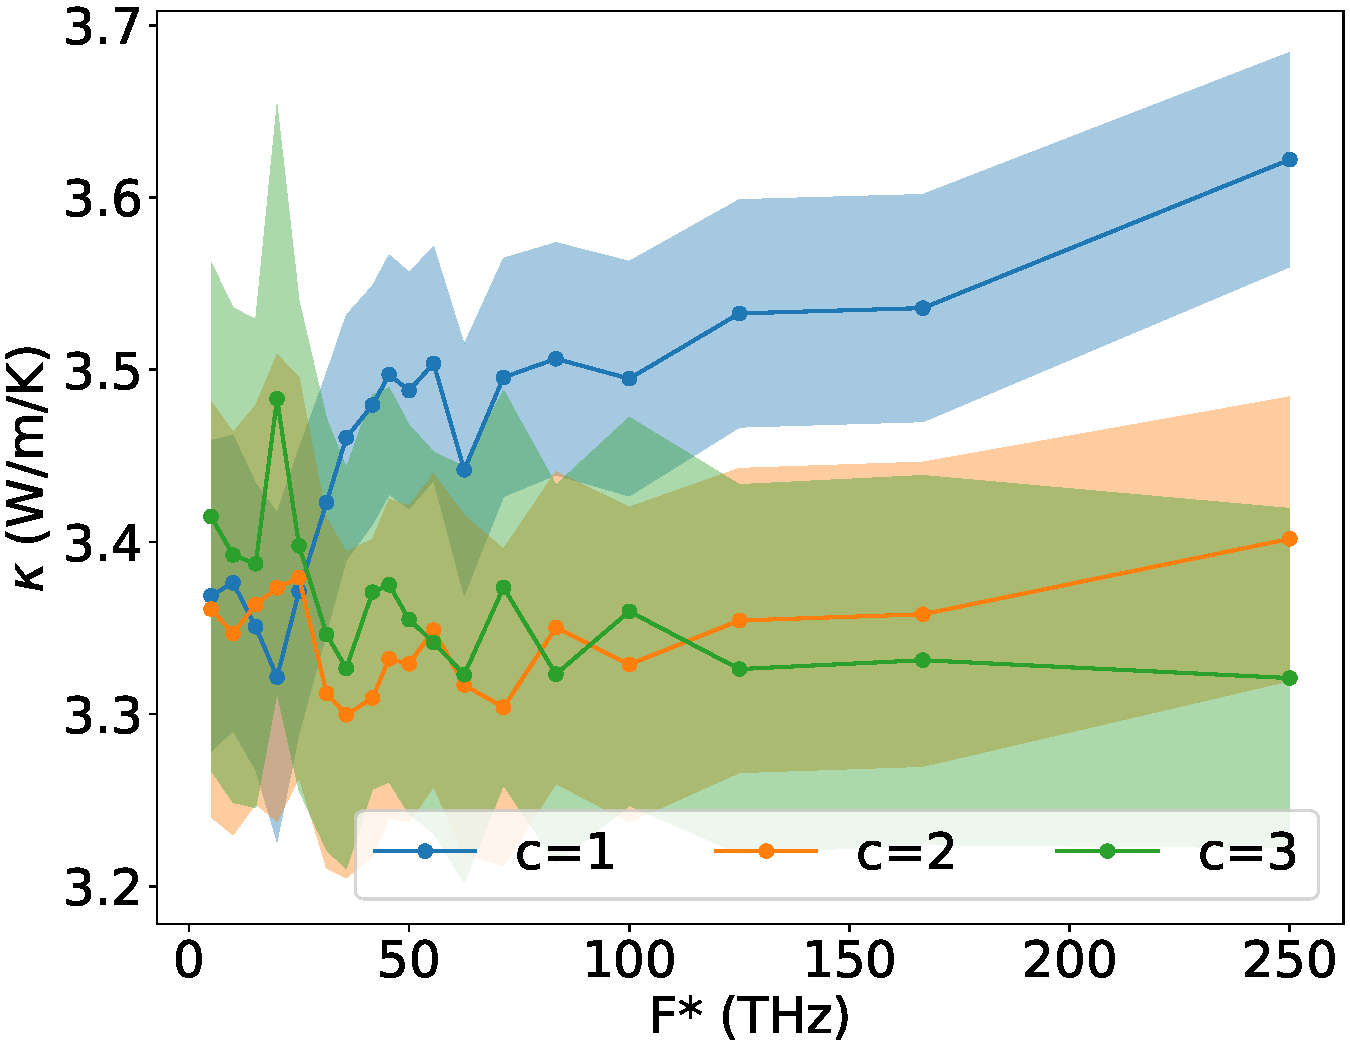
\includegraphics[width=\linewidth]{figs/kappa_corr_Fstar_1.pdf}
    \caption{Value of $\kappa$ as function  of $\FS$ for different values of $c$. }
    \label{fig:kappa1}
\end{figure}


\begin{figure}[tbh]
    \centering
    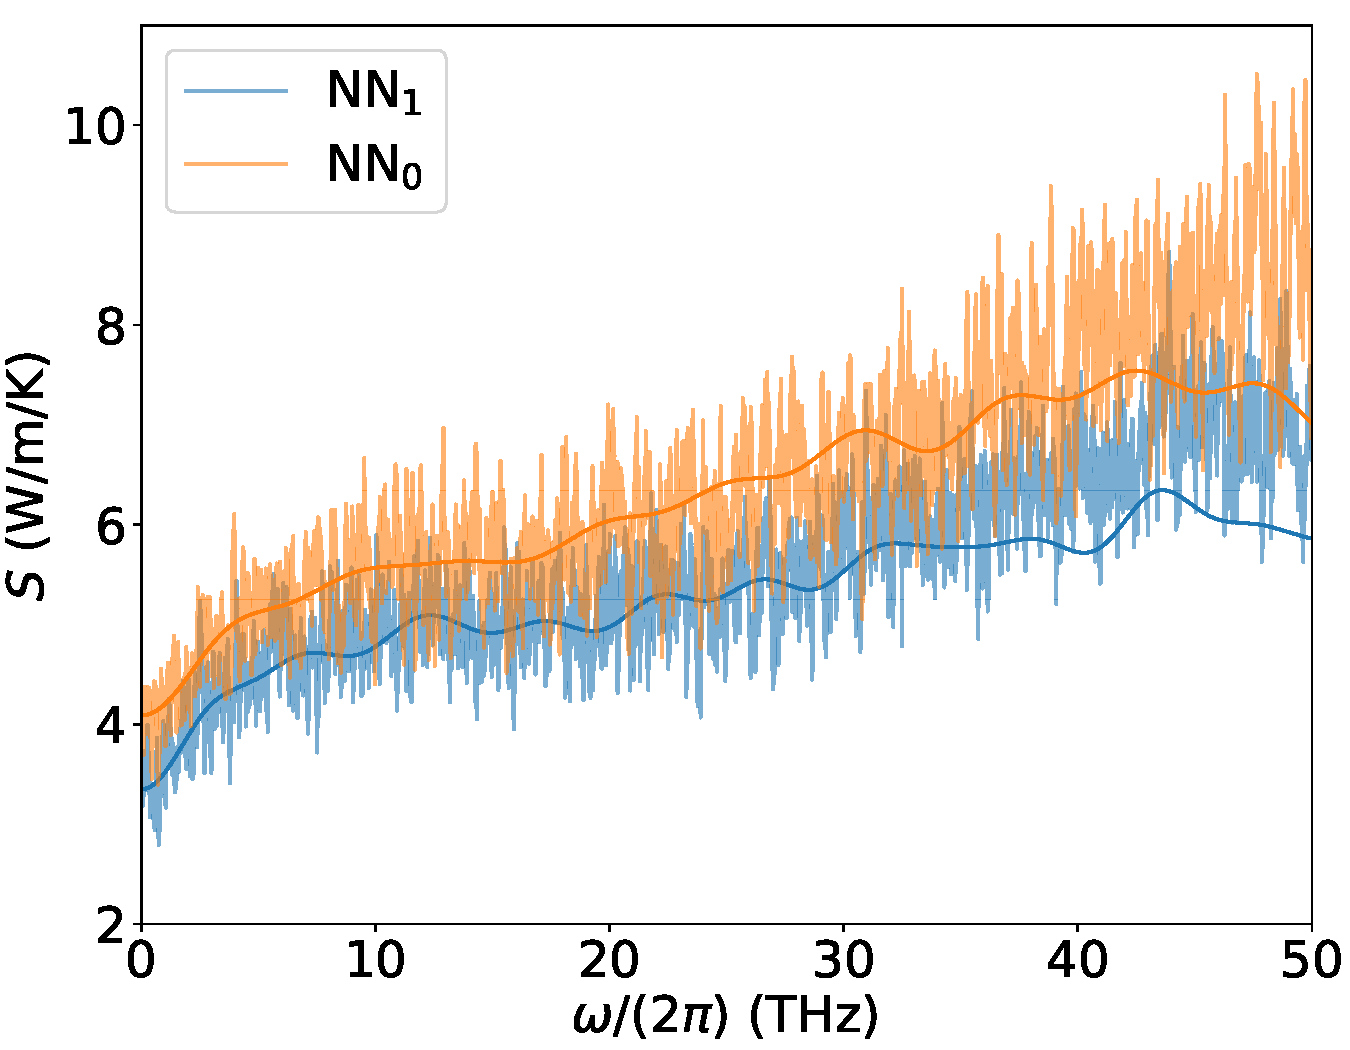
\includegraphics[width=\linewidth]{figs/Spettro_12.pdf}
    \caption{Heat spectrum for the NN$_0$ (orange lines), NN$_1$ (blue lines) trajectories. The shadowed area represent the width filter, with width equal to $0.1~$THz, of the true spectrum while the continuous line is the cepstral-filtered spectrum. $\kappa$ is estimate as the zero values of the cepstrum.} 
    \label{fig:spettri}
\end{figure}


\bibliography{apssamp}% Produces the bibliography via BibTeX.

\end{document}
%
% ****** End of file apssamp.tex ******
